\section{Results}\label{sec:results}

\subsection{An oracle near-wall band changes the field outside it}\label{sec:cube}\label{sec:first}

The foreground flow is an aligned-cube large-eddy simulation (LES) \cite{coceal2006aligned,coceal2007cubes,xie2006les} with
plan solidity $\lambda_p=0.25$ and $Re_h=5000$---exposed floor, ceiling and cube surfaces rather
than a stack of homogeneous planes (native first-cell $y^+\leq1.92$; Methods). Of 1,101
post-spin-up fields, 660 train, 98 are excluded, and 160 temporally correlated, thinned fields are
evaluated from the chronologically separated remainder. ``LES reference'' denotes this numerical record,
not ground truth: the case has no experimental benchmark or grid/filter study.

The supplied band contains 14,008 of 207,360 fluid cells ($6.8\%$; $4.5\%$ excluding two
computational-lid strips), so the complete endpoint scores 93.24\% of the fluid domain; near and
farther endpoints split the unsupplied cells at $d/h=0.5$, a geometric label, not an
equilibrium-layer claim. The intervention is rich---a dense oracle velocity band, not wall
pressure, shear or a closure output---and tests whether a conditional generator changes outside
the supplied support given time-aligned wall information. The far-time control shifts that
band by $\approx1.40$ integral times at unchanged support and density.

The chronological allocation was recorded before any wall-arm output existed (Supplementary
Note~1). Three sequential configurations of the \emph{same} three-dimensional U-Net were run, called M0, M1 and M2. They differ only in size and budget: M0 width 24 and 30,000
updates; M1 width 48, 90,000 updates and a longer sampler; M2 differs from M1 only in using
circular padding in the two periodic directions. What separates them evidentially matters more:
M0 provided the only pre-output contact with the evaluation interval, so it is the first-contact
comparison, while M1 and M2 reused that interval and are development sensitivities, not
independent confirmations.

On the complete support-excluded volume M0 gives aligned-band $\Rfluct=0.103$, against
$-0.072$ for the absent-band branch of the same network and $-0.204$ for a far-time band:
paired gains of $+0.175$ and $+0.307$, larger near the wall, with farther-from-wall absolute
skill negative (Supplementary Table~2). M1 and M2 preserve the ordering (complete gains
$0.174$, $0.197$), but the farther-from-wall paired interval crosses zero for M1, so no
model-independent outer effect is established.

\begin{table}[t]
\caption{\textbf{Valid retained controls that delimit attribution.} All values are fluctuation
$R^2$ in the complete/near/farther-from-wall regions. These later controls use the same chronological
allocation but different estimators or training protocols from M0; they are scope tests, not a
clean numerical leaderboard.}\label{tab:controls}
\centering
\small
\begin{tabular*}{\linewidth}{@{\extracolsep{\fill}}P{6.6cm}rrr@{}}
\toprule
Estimator and information & Complete & Near & Farther \\
\midrule
Linear/Wiener, no band & $-0.00008$ & $-0.00001$ & $-0.00018$ \\
Linear/Wiener, near-wall band & $-0.05068$ & $+0.02997$ & $-0.13327$ \\
Deterministic direct band, seed 2234 & $+0.05523$ & $+0.15647$ & $-0.04842$ \\
Deterministic direct band, seed 3234 & $+0.05803$ & $+0.16121$ & $-0.04762$ \\
Nearest training band, associated field & $-0.80255$ & $-0.73251$ & $-0.87430$ \\
M0 learned absent-band arm & $-0.07240$ & $-0.07669$ & $-0.06804$ \\
\bottomrule
\end{tabular*}
\end{table}
\FloatBarrier

Table~\ref{tab:controls} delimits attribution: no estimator matched to M0's architecture, budget
and selection protocol was run, so generator superiority is not established; a frozen-record
retrieval diagnostic is strongly negative in every region, rejecting literal retrieval though not
more flexible memorisation; and a support-contaminated interior comparison is quarantined
(Supplementary Note~1). The selected M2
endpoint is not an untouched held-out test.

Figure~\ref{fig:generation} makes the intervention spatially concrete. Panel \textbf{a} fixes the
first evaluated M2 target before output inspection and pairs its contemporaneous band with an
equal-support donor 172 stored fields later. Panels \textbf{b},\textbf{c} compare the LES section,
three eight-sample arm means and their absolute errors on common scales. The aligned arm reduces
error most visibly beside the floor and cube. The mean profiles remain similar (\textbf{d}), but
the wall-normal profile resolves the local difference (\textbf{e}): aligned has the lowest
near-wall error and complete-volume RMSE, $0.112$ against $0.128$ absent and $0.136$ far-time.
This is a reconstruction benefit rather than merely a shifted mean profile. Because it shows one
target from development-contacted M2, the display illustrates rather than independently tests the
aggregate result.

Figure~\ref{fig:point} separates mechanism from evidential claim. Panels \textbf{a},\textbf{b}
map where correct-time information reduces squared error: improvement clusters around the floor
and cube but is not uniform in the outer flow. Panel \textbf{c} holds the M2 U-Net and eight noise
seeds fixed while only wall information changes; panel \textbf{d} removes supplied support before
defining complete, near and farther scores, and distinguishes absolute fluctuation $R^2$ from
paired $\Delta R^2$. Panels \textbf{e},\textbf{f} then return to first-contact M0: aligned skill is
$0.103$ complete, $0.243$ near and $-0.040$ farther, while gains over absent/far-time are
$0.175/0.307$, $0.320/0.564$ and $0.028/0.044$, respectively. Thus the wall signal is strongest
near its support; the small positive farther contrasts do not produce positive outer absolute
skill. Only terminal M0 aggregates survive, so points are shown without unreplayable intervals.

\begin{figure}[t]
\centering
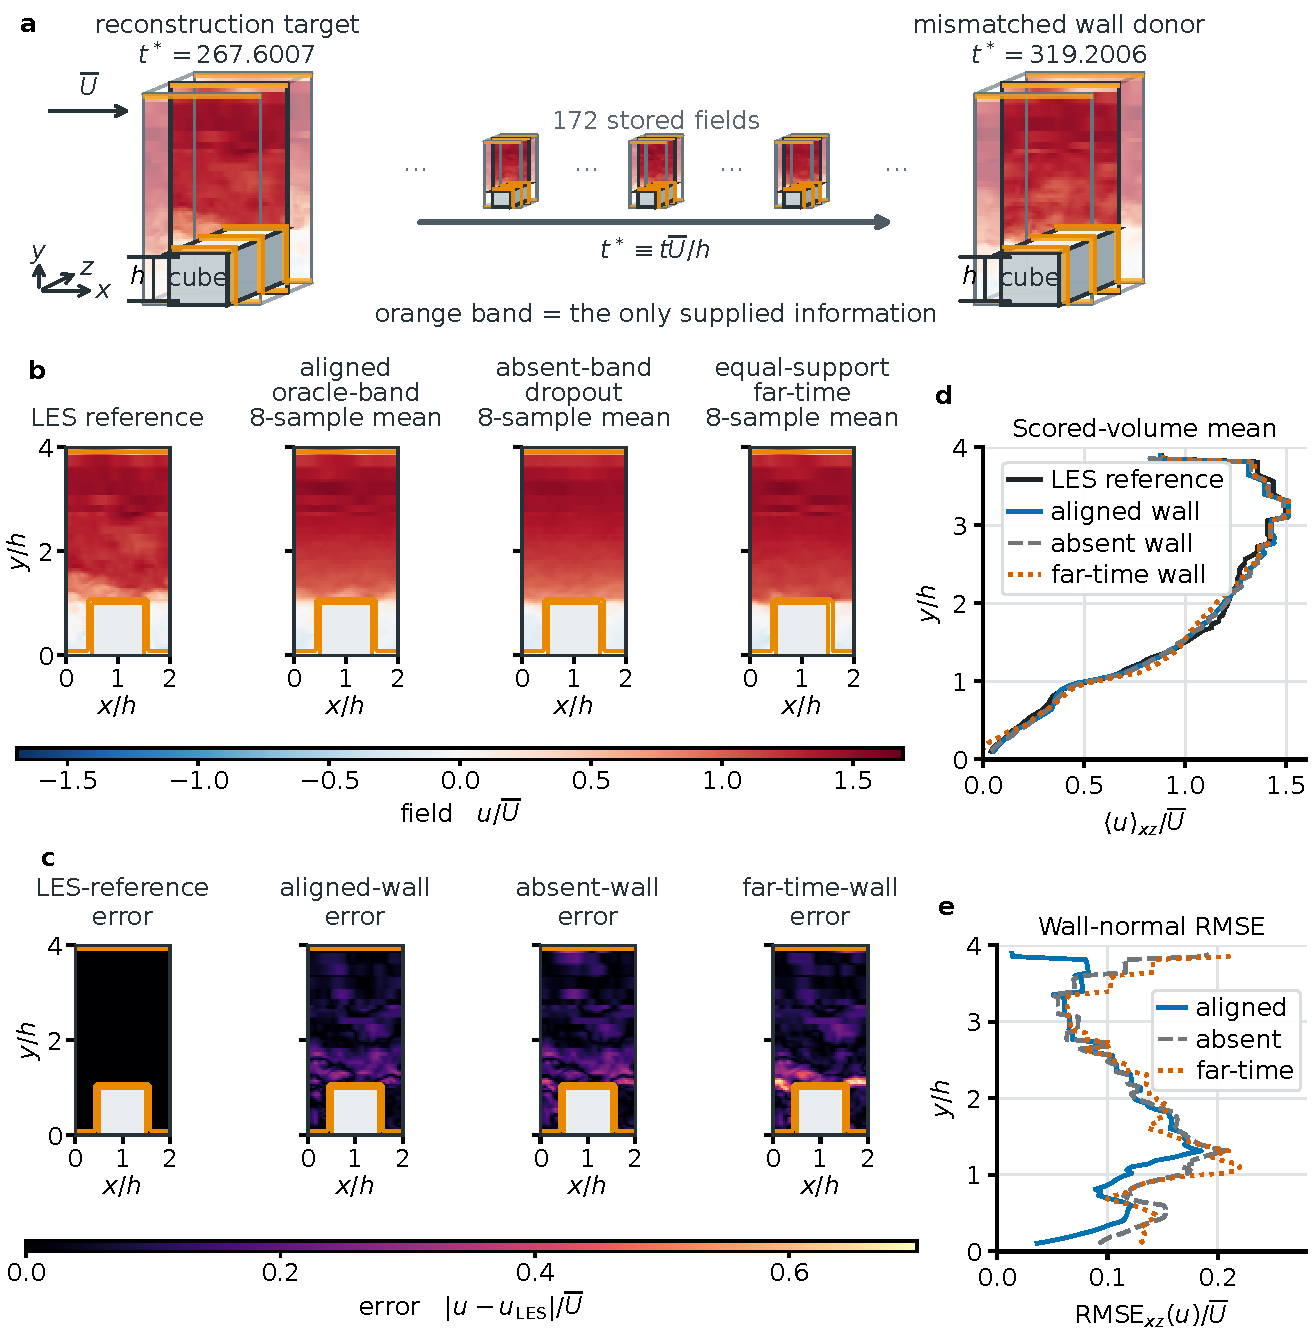
\includegraphics[width=\linewidth]{figures/fig2_generation.pdf}
\caption{\textbf{Representative aligned-cube reconstruction.}
\textbf{a}, First evaluated M2 LES target (record 758, $t\overline U/h=267.6$), fixed in
advance by the protocol rather than chosen visually, with three retained intermediate fields and
far-time wall donor (record 930); ellipses denote omitted fields. Each cutaway shows three
$x$--$y$ sections (dark: mid-span); orange marks the supplied near-wall band.
\textbf{b}, Mid-span LES reference and aligned-band, absent-band and far-time eight-sample means.
\textbf{c}, Absolute errors. \textbf{d}, Scored-volume mean profile. \textbf{e}, Wall-normal
root-mean-square error (RMSE) profile; complete-volume RMSE $0.112$ (aligned), $0.128$
(absent), $0.136$ (far-time).
One target is shown; aggregate results use 160 temporally correlated three-component fields.}
\label{fig:generation}
\end{figure}
\FloatBarrier

\begin{figure}[t]
\centering
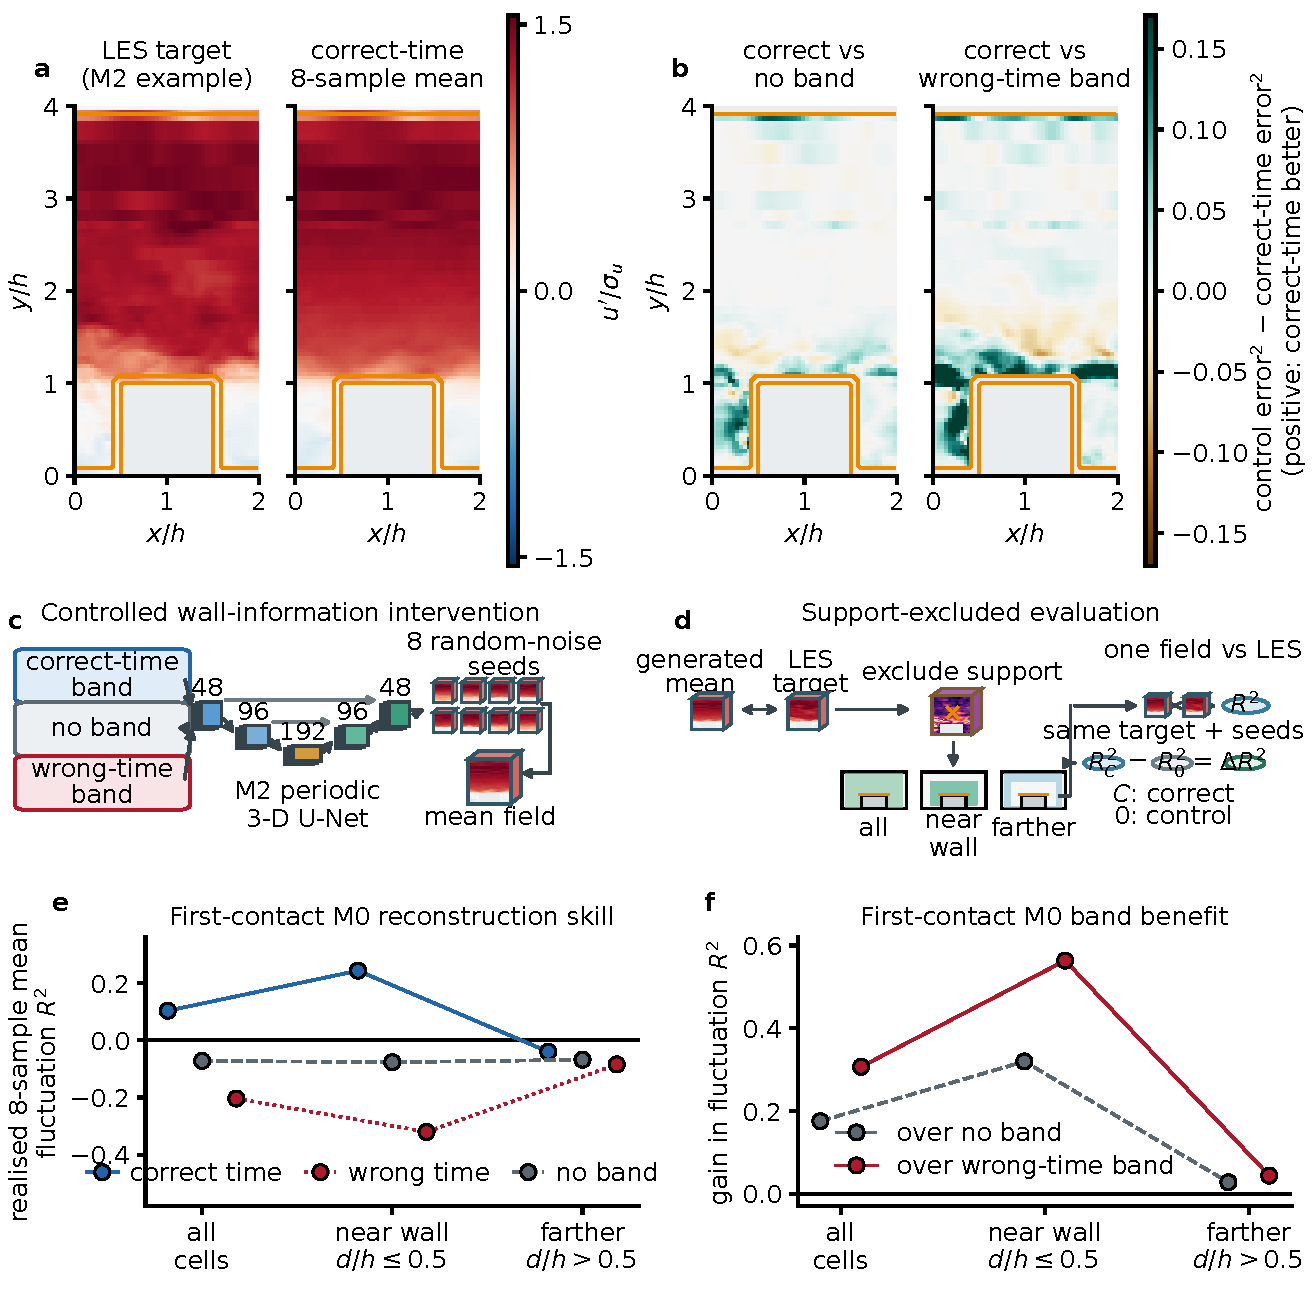
\includegraphics[width=\linewidth]{figures/fig3_propagation.pdf}
\caption{\textbf{Correct-time near-wall information acts chiefly near its supplied support.}
\textbf{a}, M2 mid-span LES target and eight-sample mean; orange marks supplied cells.
\textbf{b}, Local error reduction against no-band and wrong-time controls; green favours
correct time. \textbf{c}, Three matched arms traverse the frozen
3-D U-Net; larger cube, their eight-seed mean. \textbf{d},
All-cell, near-wall and farther masks; $R^2$ scores one arm,
$\Delta R^2$ a matched pair. Aligned, absent and far-time here score $0.120$, $-0.077$,
$-0.314$; near-wall aligned skill $0.284$. \textbf{e}, M0 field-to-LES $R^2$. \textbf{f},
Correct-time gain over controls. M0 points are terminal aggregates without replayable intervals,
but anchor interpretation as the only pre-contact comparison.}
\label{fig:point}
\end{figure}
\FloatBarrier

\emph{Post-selection distributional endpoint.} A registered farther-region energy-score
endpoint, frozen after M2 selection, favours the aligned arm over both controls ($0.522$
against $0.527$ and $0.548$)---a conditional post-selection sensitivity. \textbf{Its physical
corroboration is null}: both valid statistic families fail to beat both controls, and the
registered coverage family was withdrawn as invalid at eight members (Supplementary Note~4).

\subsection{An equilibrium velocity reconstruction destroys the interface}
\label{sec:interface}

A wall closure cannot supply a dense oracle velocity band; it supplies a signed two-component
wall traction. We first executed the standard adapter---expand that traction into a velocity band
through an equilibrium law and impose it. All arms use model M1, byte-identical to
Section~\ref{sec:first} in generator, targets, sampler noise and scoring masks; only the band
payload changes.

Two raster defects change how the published band should be read: supplied cells carrying no
information, and duplicates of scored cells. Restricting the band to the physical walls
removes both; the leak-free arm still improves on the absent branch by
$+0.102\,[0.093,0.109]$, so the computational ceiling accounts for about
42\% of the published $+0.174$ gain (Supplementary Note~3).

Against that matched ceiling the traction interface fails (Fig.~\ref{fig:interface}). The
target-velocity equilibrium inversion through the frozen lift scores $-0.117$ on the complete
volume, a change of $-0.032\,[-0.048,-0.021]$ relative to supplying nothing, and its transmission
ratio against the matched ceiling is $-0.320\,[-0.517,-0.194]$. The controls locate the failure: the traction is not information-free---the instantaneous
inversion beats the mean wall load and a far-time traction ($+0.199\,[0.162,0.239]$)---yet every
lifted arm sits below the absent branch (Fig.~\ref{fig:interface}b,c). The a-priori diagnostic explains why: the lifted
band reproduces the true band with fluctuation
$R^2=-0.109\pm0.185$, worse than the band's own mean, and the sampler clamps that error into the
field along the whole trajectory (Eq.~\eqref{eq:hard}).

This bounded negative falsifies only the composition tested. Two confounds live in the adapter,
not in the wall information: the lift is an equilibrium model of an instantaneous field, and
every lifted arm is outside the frozen generator's conditioning distribution. The next
subsections remove it.

\begin{figure}[t]
\centering
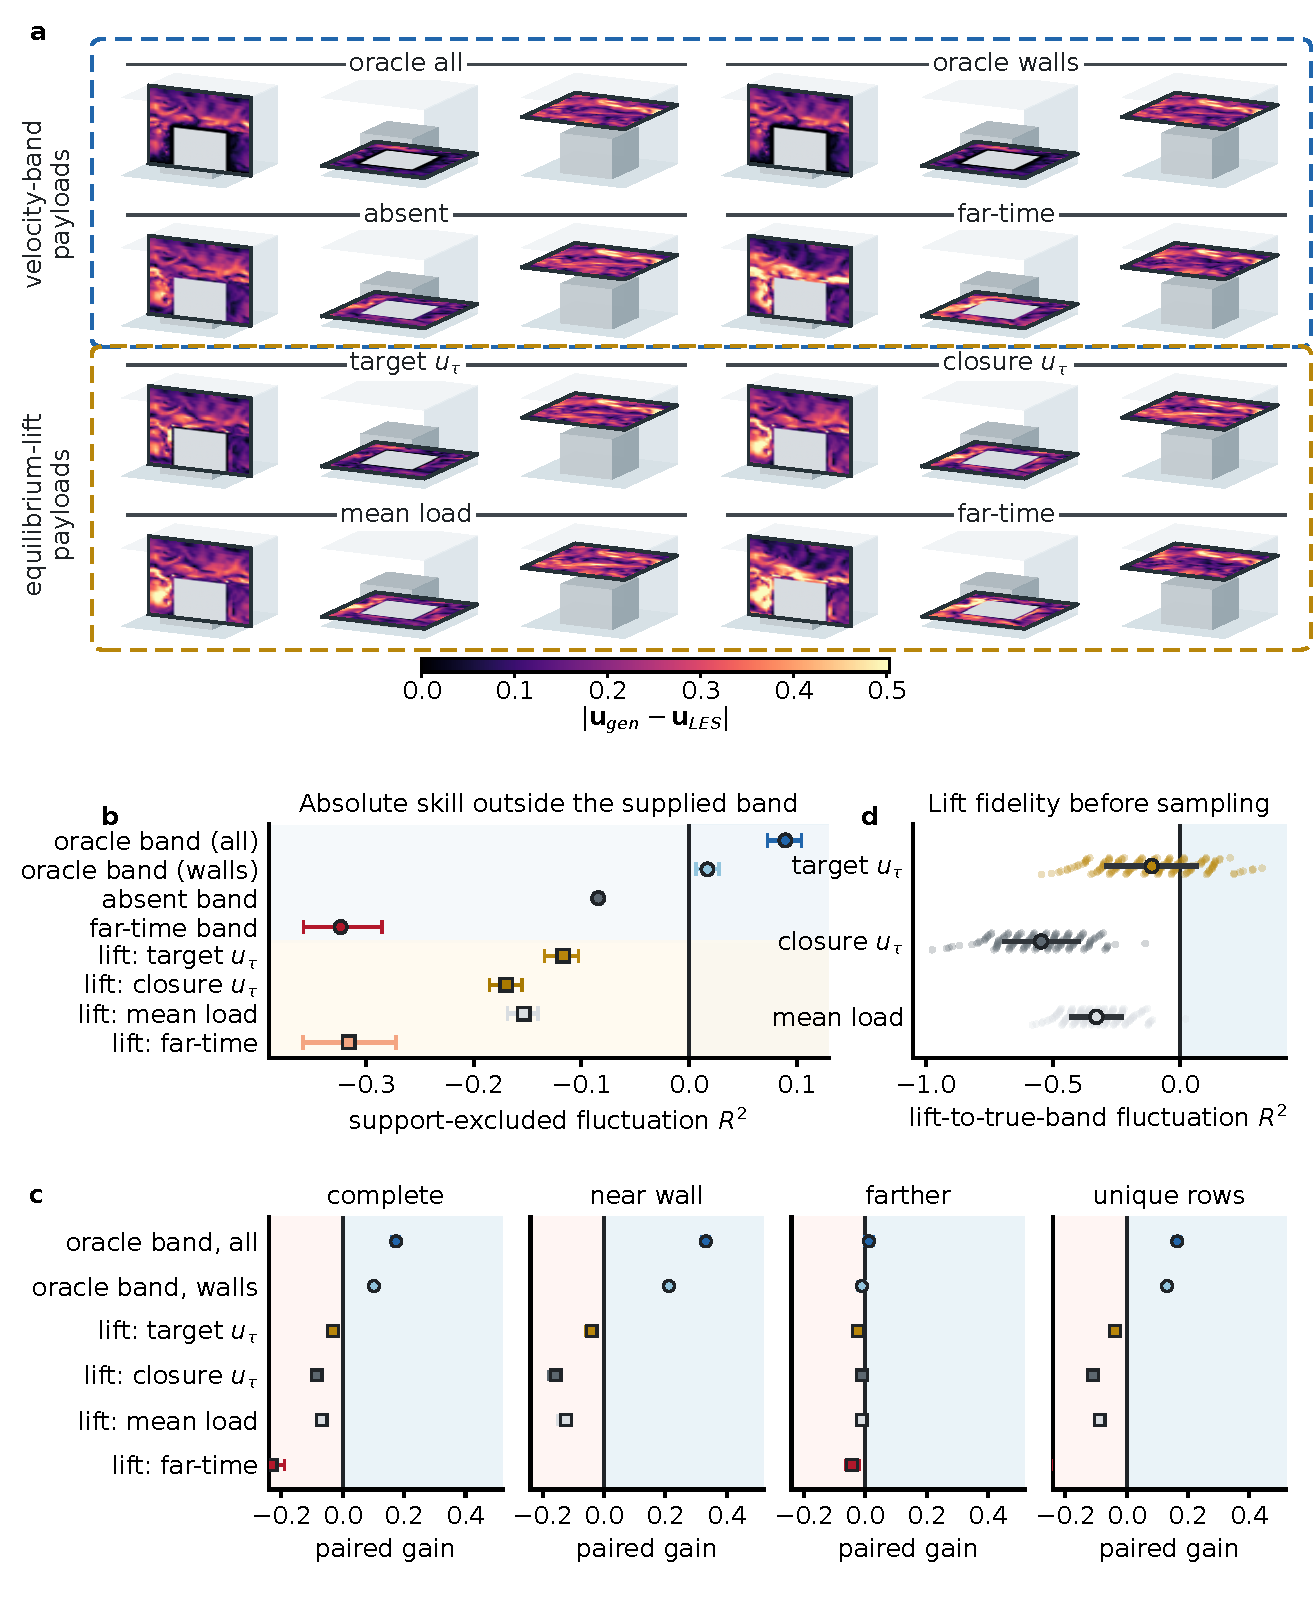
\includegraphics[width=\linewidth]{figures/fig6_interface.pdf}
\caption{\textbf{Frozen closure-to-generator interface.}
Only payload changes. \textbf{a}, Representative 3-D errors for eight payloads on mid-span,
near-wall and outer planes. \textbf{b}, Support-excluded $R^2$; a model-predicted traction with
no target-derived wall information (friction-velocity field correlated $0.782$ with the
inversion) scores $-0.085\,[-0.098,-0.073]$, and the instantaneous inversion beats the mean
wall load by $+0.037\,[0.021,0.054]$. \textbf{c}, Gain over absence by
region; whiskers in \textbf{b},\textbf{c} are conservative 95\% intervals. \textbf{d}, Target-wise
lift fidelity (mean $\pm$ s.d.). Oracle bands help; every lifted-traction arm underperforms
absence. This result covers only the frozen lift--generator composition, not general wall closures
or solver-coupled performance.}\label{fig:interface}
\end{figure}
\FloatBarrier

\subsection{A first-cell wall traction propagates without any velocity reconstruction}
\label{sec:direct}

Removing the adapter requires conditioning on the surface quantity itself. The tangential
projector annihilates the isotropic pressure term (Eq.~\eqref{eq:traction}), so a wall-on-fluid
traction is recoverable from the velocity record alone
(Eq.~\eqref{eq:nativetau}): a \emph{first-cell viscous traction} on the model raster, not the
native spectral-element derivative. Physical consistency checks ran before any arm was sampled
(Methods). Generators were then trained from scratch to condition directly on that traction---no velocity
reconstruction, no clamp---under a protocol frozen and hash-bound before the production run,
which discloses prior contact: a previously contacted record, not an untouched confirmation
($N_{\mathrm{eff}}=2.46$).

The contrast is positive in every scoring region (Fig.~\ref{fig:direct}). On the complete
unsupplied volume the first-cell traction improves support-excluded fluctuation $R^2$ by
$+0.074\,[0.070,0.078]$ over the absent-conditioning branch, with the same sign on all three
seeds (across-seed s.d. $7.52\times10^{-4}$); the near-wall gain is $+0.140\,[0.135,0.145]$,
decaying outward (Fig.~\ref{fig:direct}e). Against a matched ceiling---the oracle band on the same support, retrained identically
($+0.117\,[0.111,0.123]$)---the traction transmits $0.631\,[0.622,0.639]$.

The controls place the effect in the wall information, not the act of conditioning: the traction
arm beats a training-window mean load, a far-time, a shuffled and a sign-reversed traction by
$+0.077$ to $+0.204$ on the complete volume (Fig.~\ref{fig:direct}d). The shuffled and
sign-reversed fields are out-of-training inputs measuring sensitivity under distribution shift,
so the signed orientation is not by itself established as causal.
One contrast runs the other way: farther from the wall the sign-reversed arm beats the correct
one by $0.022\,[0.011,0.032]$.

Three limits bound this. The traction is read from the held-out target, so it measures what a
closure's output could transmit---closure accuracy is the question Sec.~\ref{sec:closurecomp}
answers. It is an invertible linear map of the first-cell tangential velocity
(Eq.~\eqref{eq:nativetau}), strictly less informative than the band, so a transmission ratio
below one is not by itself evidence of a lossy interface. And absolute skill remains negative
($-0.014$ against $-0.088$ for absence). 

\begin{figure}[!htbp]
\centering
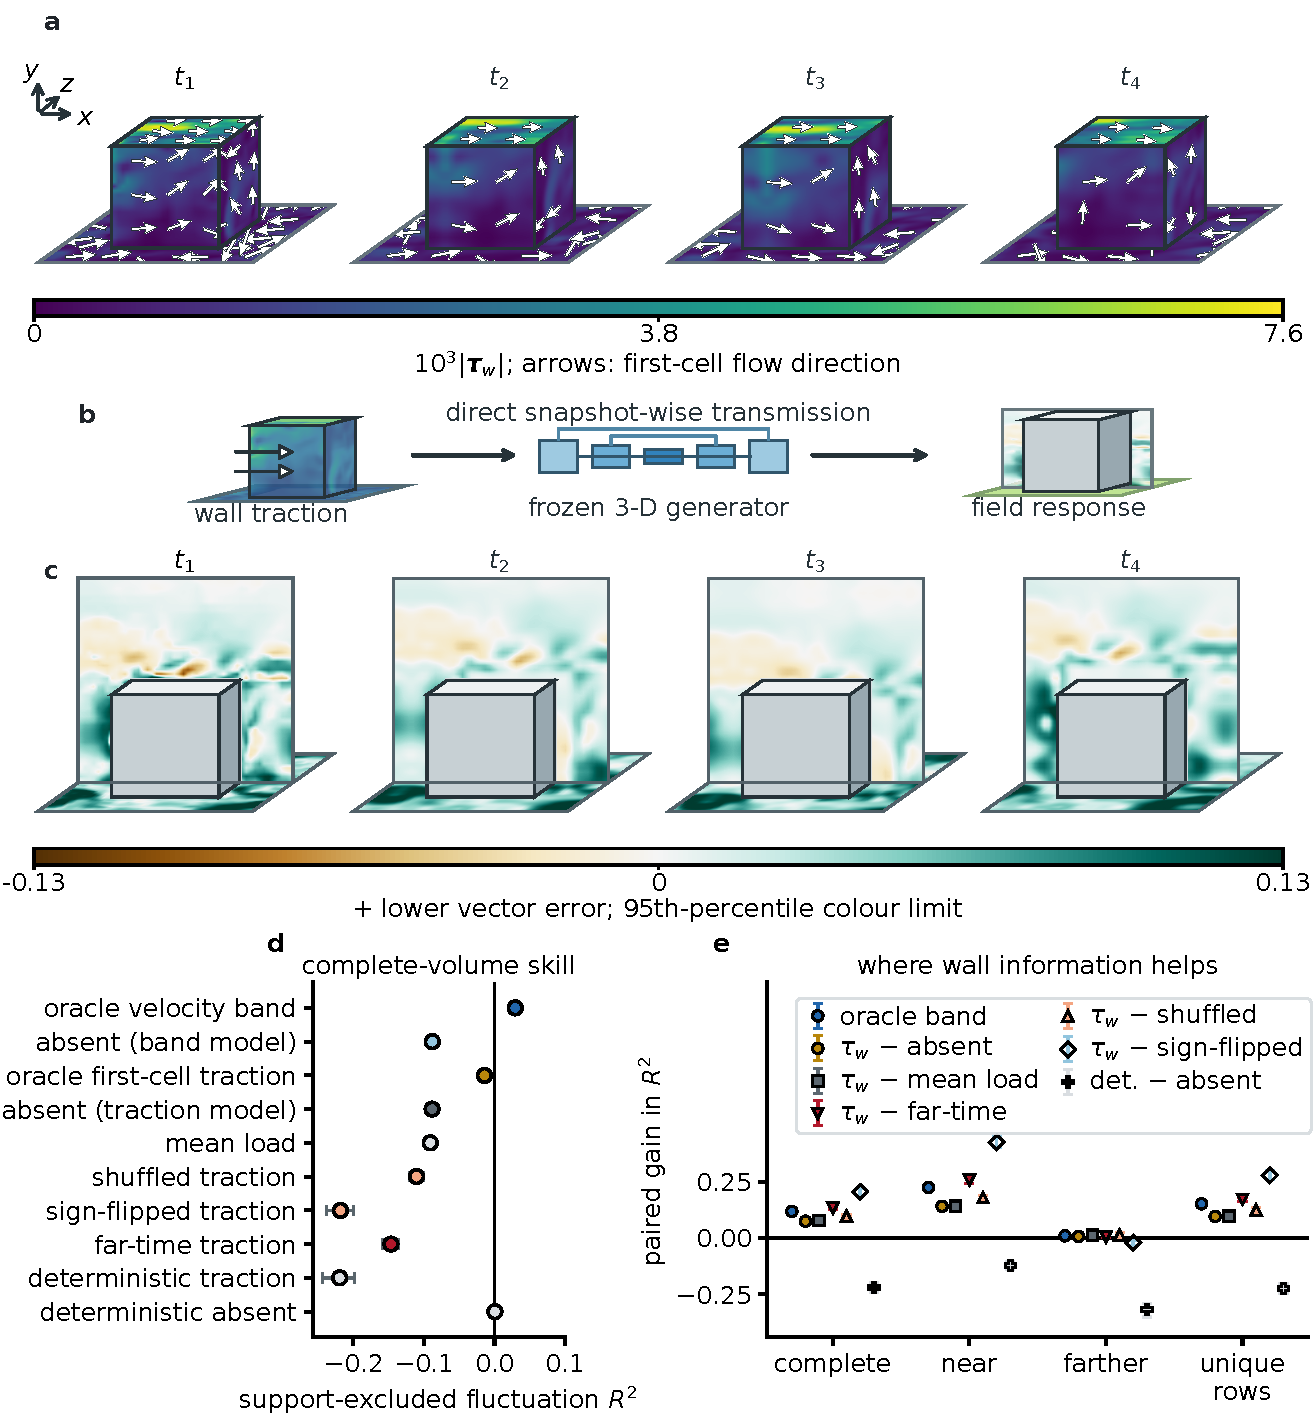
\includegraphics[width=\linewidth]{figures/fig7_direct_traction.pdf}
\caption{\textbf{Direct traction retains useful near-wall information.}
\textbf{a}, Wall-traction magnitude and first-cell flow direction at four illustrative instants.
\textbf{b}, Snapshot-wise transmission through the frozen 3-D generator.
\textbf{c}, Near-wall and midspan vector-error reduction (green indicates improvement).
\textbf{d}, Complete-volume skill across controls.
\textbf{e}, Paired gains across four regions; open markers denote out-of-training probes.
Intervals use conservative moving blocks. The traction is oracle---an invertible linear map
of the first-cell tangential velocity---and evaluated offline.}
\label{fig:direct}
\end{figure}
\FloatBarrier

\subsection{A closure that never sees the wall propagates into the field}
\label{sec:closurecomp}

Here we close the last map. A closure is fitted on the training window alone,
frozen by hash, and used to \emph{predict} held-out signed wall traction from matching-height
outer-flow state only---velocity at $2.5\Delta$ and
$4.5\Delta$ from each face, the wall-modelled-LES seam a coarse solver carries. It
never reads the wall-adjacent cell (Sec.~\ref{sec:closuremethodfit}), and its prediction is
all the generator receives. The score excludes every supplied cell \emph{and} every closure-read cell (8,040 more), with the
registered rule evaluated on 103 hash-bound held-out frames outside the direct-traction
experiment's index, prospectively unscored with prior contact recorded (Supplementary Note~1).

\emph{The closure.} On those frames the closure predicts the first-cell traction with
zero-traction-reference skill $0.540$ and mean direction cosine $0.746$, against $0.413$ for the
classical equilibrium wall model it contains as the case $a=\theta=0$
(Fig.~\ref{fig:closurecomp}e,f). The statistic normalises mean squared error (MSE) by the training-window root-mean-square rather than centring it
(both conventions in Sec.~\ref{sec:reachgated}); fit, validation and held-out scores are
$0.553$, $0.539$ and $0.540$, consistent with a 5,426-parameter correction that has not
overfitted.

\emph{The composition.} Conditioning the generator on that predicted traction improves
source-excluded fluctuation $R^2$ by $+0.061\,[0.057,0.064]$ over the absent-conditioning branch
of the same network, with the same sign on all three seeds and a crossed seed$\times$block
interval of $[0.055,0.065]$ that also excludes zero. The gain is $+0.118\,[0.112,0.124]$ near the
wall and positive under all seeds farther out (Fig.~\ref{fig:closurecomp}h).
All five registered clauses pass, computed mechanically from the released decision-rule record.
This is the paper's central claim: a wall quantity a closure actually produces---not one read
from the answer---propagates into the surrounding field.

\emph{Controls.} The decisive control is a far-time traction---a genuine traction of the wrong
instant, and a training class of this generator, so no distribution-shift confound. It is
\emph{worse than supplying nothing} ($-0.043\,[-0.053,-0.030]$), and the closure beats it by
$+0.104\,[0.092,0.114]$: wall information helps only at the right instant. A mean-load, a
shuffled and a sign-reversed traction are also below absence
(Fig.~\ref{fig:closurecomp}h).

\emph{Where the gain comes from.} At matched input information the learned non-equilibrium
correction is worth $+0.013\,[0.003,0.021]$ over the pure equilibrium closure, and the closure
arm exceeds the oracle traction arm by $+0.013\,[0.003,0.021]$---not prediction beating truth,
since the arms carry \emph{different} information and a closure's matching-height view is at
least as useful for propagation as an exact wall derivative. Complete-volume absolute skill
nevertheless remains negative for every arm ($-0.028$ closure against $-0.088$ absence, $-0.041$
oracle, $-0.131$ far-time).

\emph{Distributional validation.} The closure arm has the lowest continuous ranked probability
score (CRPS), per-cell energy score
and rank-histogram reliability deviation of any arm at every ensemble size
(Fig.~\ref{fig:closurecomp}d): the improvement is distributional, not an artefact of averaging.

\emph{A bounded engineering consequence.} The streamwise viscous wall force inferred from the
generated field---an offline reconstructed first-cell diagnostic excluding pressure and form
drag, not the traction a solver would consume---falls in relative RMSE from $0.099$ to $0.061$
with the closure, its correlation with the true load rising from $-0.178$ to $+0.741$
(Fig.~\ref{fig:closurecomp}g). The equilibrium closure is \emph{worse} than absence here despite
a similar field-$R^2$ gain: the learned correction matters far more for wall load than for
volume-averaged skill.

\emph{Transfer and non-regression.} The frozen generator of Sec.~\ref{sec:direct}, reused
byte-for-byte, gains $+0.036\,[0.024,0.046]$ from the predicted traction against $+0.052$ for
the oracle traction it was trained on---about seven-tenths, the expected cost of feeding a
predicted signal to a model trained on measured ones. Replaying the frozen checkpoints on that
experiment's exact frames reproduces its published values within the frozen $0.005$ identity
tolerance, and all eight prospectively frozen tolerances pass.

\begin{figure}[!htbp]
\centering
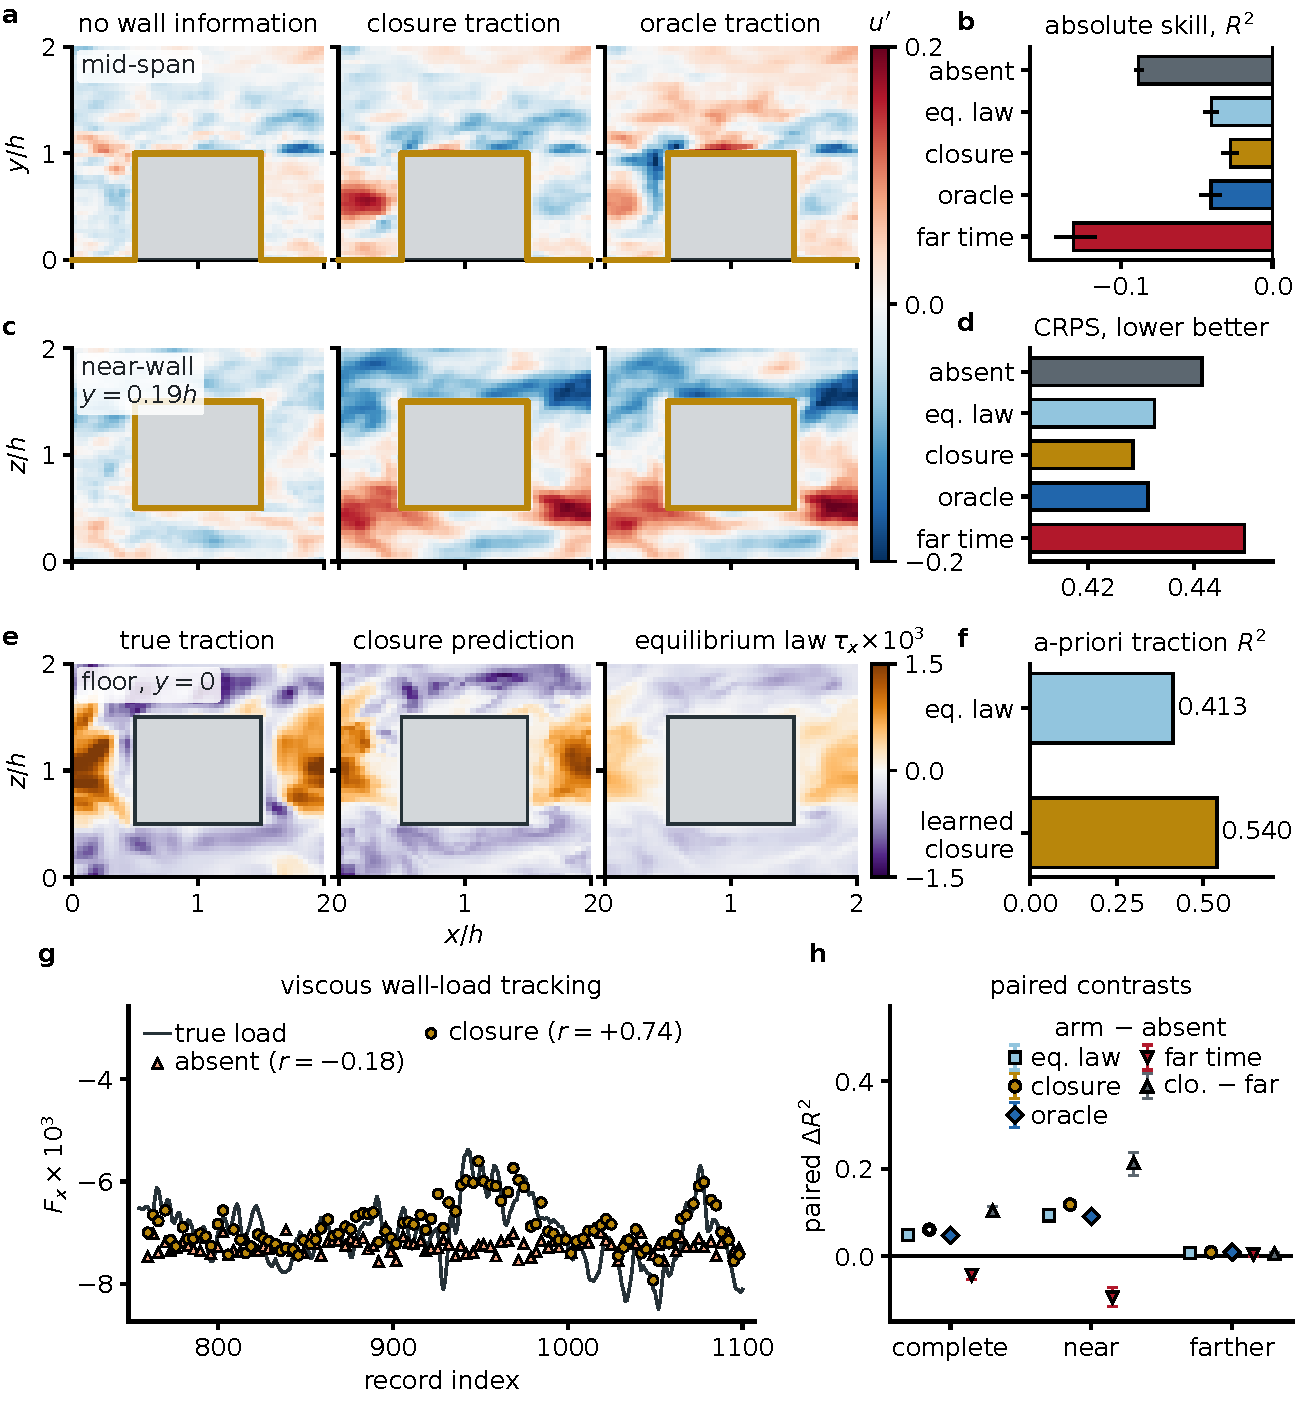
\includegraphics[width=\linewidth]{figures/fig8_closure_composition.pdf}
\caption{\textbf{A physics-grounded wall closure supplies traction that propagates through the
generative model.} \textbf{a},\textbf{c}, Posterior-mean streamwise fluctuation of held-out
record 760, mid-span and near-wall ($y=0.19h$): absent, closure, oracle traction;
gold marks traction-carrying walls. \textbf{b},\textbf{d}, Absolute source-excluded skill
(every arm negative) and CRPS; closure-arm energy score $0.922$ against $0.948$
(absent), reliability deviation $0.146$ against $0.165$. \textbf{e}, Floor
traction: true, closure-predicted, equilibrium. \textbf{f}, A-priori traction skill.
\textbf{g}, Implied viscous wall force vs true load (oracle: relative RMSE $0.035$,
correlation $+0.927$; equilibrium $0.160$, bias $+0.147$). \textbf{h}, Registered paired
contrasts; open circles, seeds. Scored on 103 prospectively unscored frames, outside every
supplied and closure-read cell; offline.}\label{fig:closurecomp}
\end{figure}
\FloatBarrier

\subsection{The interface transmits on a separating flow}\label{sec:generality}

The cube wall is geometrically pinned. To ask whether the composition survives a wall whose
stress is set by the flow, the identical protocol was re-executed on the \emph{separating
periodic-hill} flow \cite{frohlich2005highly,breuer2009hill,xiao2020hills} at $Re_h=2800$ in both
generative families and at two rasters, together with the cube under a \emph{denoising-diffusion}
generator \cite{ho2020ddpm}. The hill wall is smooth and curved, with
pressure-gradient-induced separation---the regime where equilibrium wall models fail
(Fig.~\ref{fig:reachgated}a--c). It is a 2-D $(u,v)$ corpus with no spanwise dynamics.

Two properties of the protocol travel to any wall-to-field study.
\emph{The evaluation unit is the physical time, not the stored array}: this corpus stores three
spanwise planes per physical time, correlated up to $0.996$, so scoring groups planes by physical
time and separates training from scoring by $110$ of them. A flattened array-index split instead
hands each test frame its own same-time twins during training, inflating $R^2_{\rm fluct}$ by
$0.839$ (Supplementary Note~10). And \emph{a unit must show it can detect wall information before
it may adjudicate the interface}: no conclusion is drawn unless conditioning on true near-wall
information improves reconstruction with an interval excluding zero. A contact audit
shows no physical time of this record is untouched by earlier analyses, ours included.

The record passes that control in the diffusion family, and so does the method. Supplying the
traction \emph{directly}---the surface quantity the generator was trained to read---the record's
own exact direct-numerical-simulation (DNS) traction improves source-excluded fluctuation $R^2$
by $+0.058\,[+0.009,+0.107]$, and the traction predicted by the frozen closure, which never reads
a wall-adjacent cell, improves it by $+0.062\,[+0.017,+0.106]$, both proper scores agreeing
(CRPS $-0.0124\,[-0.0188,-0.0056]$; energy score $-0.0172\,[-0.0268,-0.0076]$). Two paired
contrasts say what that gain is made of: the closure arm is not resolved from the exact
traction ($+0.004\,[-0.007,+0.017]$)---no advantage of the wall truth over the fitted closure
is detected here; and the traction signal is \emph{read} rather than merely present, the
closure arm beating the same traction from a wrong instant by $+0.045\,[+0.001,+0.086]$ over the
volume and $+0.101\,[+0.017,+0.170]$ near the wall, where wrong-instant information falls
\emph{below} supplying nothing.

The bounds matter as much. The near-wall interval for the closure arm alone crosses zero
($+0.063\,[-0.022,+0.152]$), and the arm is separated from neither a magnitude-matched scrambled
traction ($+0.026\,[-0.021,+0.067]$) nor the equilibrium law ($+0.011\,[-0.015,+0.031]$), so
specificity holds against wrong timing but is unresolved against wrong spatial pattern; absolute
skill stays negative for every arm. With $370$ scored times against a measured integral time of
$112.3$, $N_{\rm eff}\simeq3.3$: every hill interval here, favourable and adverse alike, is
indicative rather than precise, and the hill is not part of this paper's headline claim.

How the traction is presented decides whether it transmits. Expanding it first into a near-wall
velocity band through the closure's Reichardt profile does \emph{not} clear zero at either raster
($+0.038\,[-0.017,+0.091]$ at $64\times192$; $+0.059\,[-0.011,+0.122]$ at $96\times288$), despite
that lifted band reproducing the true band velocities at $R^2=0.871$ and $0.915$ and the
equilibrium lift matching it to three decimals: fidelity in the lifted representation is not
sufficient. The oracle band arm, which \emph{is} the record's exact band rather than a lift, does
pass at both rasters ($+0.057\,[+0.011,+0.107]$ and $+0.079\,[+0.027,+0.131]$;
Fig.~\ref{fig:reachgated}f); its scrambled control is itself weakly positive over the whole
volume ($+0.018$), so part of any whole-field gain is non-specific, but near the wall that
vanishes and wrong information falls below absence.

At the wall the record is positive in both families. The closure predicts wall traction on the
time-disjoint unit with $R^2=0.757$, against $0.557$ for the equilibrium law it contains
(Fig.~\ref{fig:reachgated}d), and conditioning on it improves the reconstructed wall force
($0.036\to0.542$ and $-0.104\to0.445$ in correlation)---an offline reconstructed first-cell
viscous-force diagnostic excluding pressure and form drag. The wall quantity is recovered even
where the outer field is not: the near-wall/whole-field dissociation volume-averaged objectives
conceal. The flow-matching cell fails the same positive
control at both rasters, so by the standing rule it cannot adjudicate the interface in either
direction; that arm and its failed repair are treated in the
Discussion. Every registered contrast, sampler, raster and control is
tabulated in Supplementary Note~10, with two further checks that fail their preregistered
criteria, the withdrawn composition attempts and the custody audit that forced refitting the
closure on the cube record (Supplementary Notes~6--8).


\subsection{A re-test on a record that passes the control shows the interface transmits, and how
far}
\label{sec:reachgated}

To decide the whole-field question on a unit with demonstrated detectability, we re-executed the
frozen closure$\rightarrow$traction$\rightarrow$generator composition on the wall-resolved cube
record with three changes fixed before any outcome existed (Supplementary Note~11): the split is
\emph{reversed in time}, everything refitted from scratch on late frames and scored on a
never-tested $25$-frame window $132$ frames from training; both families are trained at an
identical budget with one frozen conditioning mixture including the oracle band, so band and
traction arms are compared \emph{within one propagator}; and the near-wall region $d\le0.5$ is
co-primary with the whole field. That region is outcome-informed, hence evaluated on a fresh unit.

The positive control passes in both families ($+0.130\,[0.115,0.145]$ and
$+0.029\,[0.026,0.032]$; Fig.~\ref{fig:reachgated}g), and so does the interface. Conditioning on
traction predicted by a closure that never reads a wall-adjacent cell raises near-wall
fluctuation $R^2$ from $-0.098$ to $+0.005$, a gain of $+0.103\,[0.091,0.115]$
(Fig.~\ref{fig:reachgated}h)---the first arm here with positive absolute skill, recovering
$79\%$ of the DNS-band ceiling in the same propagator. The matched controls
separate cleanly: a spatially shuffled traction of identical support and magnitude multiset
scores $-0.128$ and a wrong-instant field $-0.164$, both \emph{worse} than supplying
nothing---the generator reads arrangement and instant, not the presence of a channel.

The effect has the wall-normal structure a boundary condition must have
(Fig.~\ref{fig:reachgated}i): in nested shells the same frozen contrast decays monotonically from
$+0.266\,[0.221,0.317]$ at $d\le0.15$ to $+0.006\,[0.004,0.008]$ beyond $d>0.5$, the nearest
scorable shell reaching $R^2=+0.149$ absolute against $-0.117$ unsupplied. The gain is $5.0$ times
larger beside the wall than in the whole-field average and $46$ times larger than in the outer
region, while the whole-field gain, $+0.053\,[0.046,0.063]$, replicates the registered $+0.061$
of Sec.~\ref{sec:closurecomp} on an independent, reversed-time unit.

Because the decisive window has $N_{\rm eff}=1.21$, the claim does not rest on the interval:
the paired per-frame difference is positive in $25$ of $25$ held-out frames for both
flow-matching seeds (minimum $+0.042$; diffusion $25/25$ and $24/25$;
Fig.~\ref{fig:reachgated}j).

The engineering-facing consequence is the reconstructed first-cell \emph{viscous} wall
force, an offline surrogate excluding pressure and form drag: closure conditioning moves its
correlation with the true load from $-0.14$ to $+0.51$ (Fig.~\ref{fig:reachgated}k;
Supplementary Note~11). One adverse detail is reported: the shuffled control attains a
\emph{higher} wall-force correlation ($+0.61$), mechanically, since permuting whole traction
vectors leaves the integrated force invariant---this integral cannot discriminate arrangement
while the field endpoint does.

Two limits are registered rather than argued away. The rule frozen before this run returns
\textbf{fail} on one clause---the diffusion family's \emph{absolute} unconditional skill,
$-0.53$, does not reach the inherited $-0.14$ floor, even though its interface delta is positive
and interval-separated; a development sweep locates that in the family's posterior mean rather
than in the interface, and the threshold was not adjusted after the outcome. And while the
closure captures the held-out traction pattern better than the equilibrium law
(Fig.~\ref{fig:reachgated}e), the instantaneous departure from the held-out mean traction remains
largely unpredicted (Supplementary Note~11).

As in Sec.~\ref{sec:closurecomp} the closure arm slightly exceeds the \emph{oracle traction} arm
($+0.005$ versus $-0.015$); the oracle band remains above both.

\begin{figure}[t]
\centering
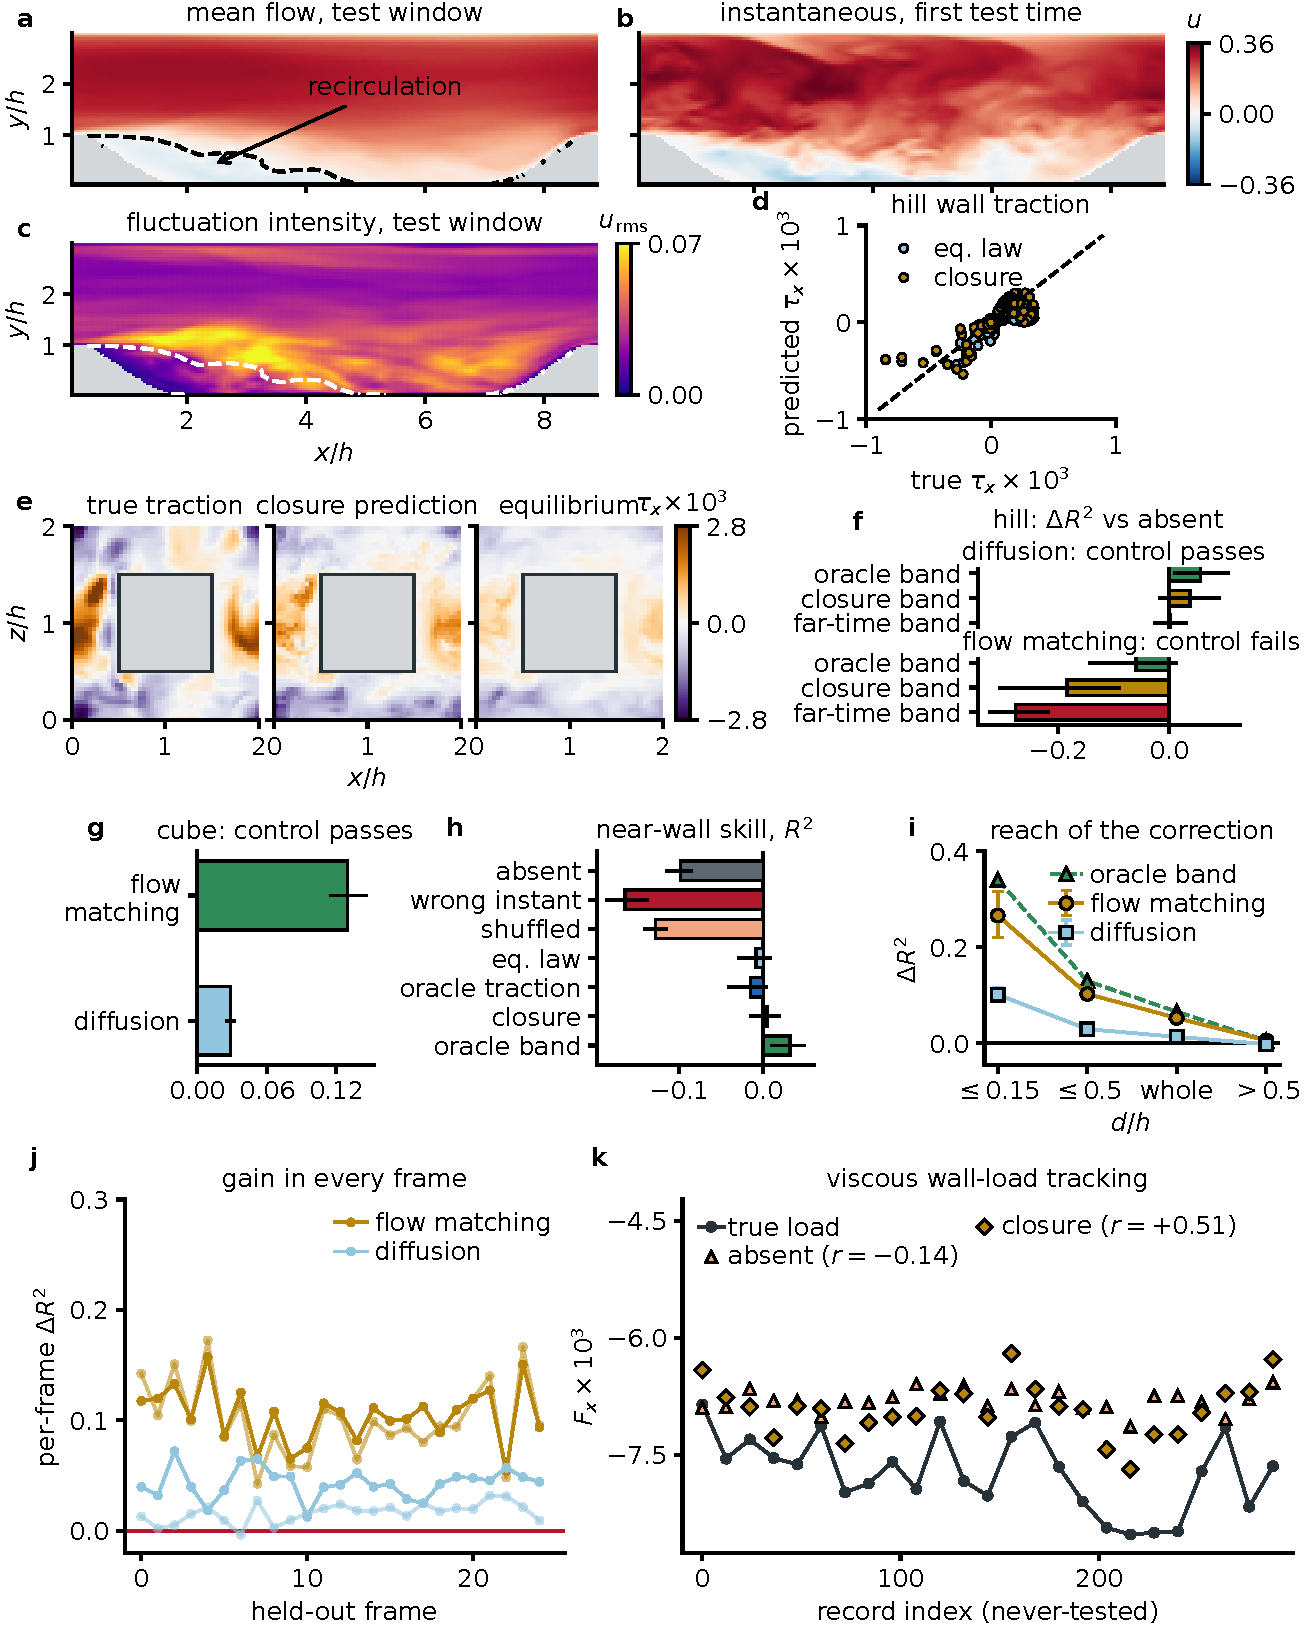
\includegraphics[width=\linewidth]{figures/fig11_reachgated_composition.pdf}
\caption{\textbf{A prospectively frozen oracle positive control decides which cells may
adjudicate the interface.} \textbf{a}--\textbf{c}, Separating hill: test-window mean flow
(dashed, $\bar u=0$), an instantaneous frame, shear-layer fluctuation intensity.
\textbf{d},\textbf{e}, Held-out traction on the separating wall and a never-tested cube frame.
\textbf{f}, Each band arm's paired contrast against its own absent branch at $64\times192$; the
label gives that family's \emph{positive-control} verdict, not a verdict on the closure arm. The
flow-matching failure survives a stochastic sampler and a finer raster (Supplementary Note~10).
\textbf{g},
Positive control on the reversed-time cube. \textbf{h}--\textbf{k}, Near-wall ladder; reach
against ceiling; per-frame gain; viscous wall-load tracking. All endpoints offline.}
\label{fig:reachgated}
\end{figure}
\FloatBarrier

\subsection{A single-slot channel experiment measures what transmitted traction is worth}
\label{sec:slot}

Earlier generators saw named wall-signal classes during training. A prospectively registered
single-slot experiment on a second, wall-resolved
record---the smooth-wall channel of the public CoNFiLD release at
$Re_\tau=184$---removes that asymmetry. The generator is trained on exactly one
traction-carrying condition, the record's own signed traction under a variance-preserving
fidelity ladder, so every wall model enters the same slot with zero generator-side training
exposure. A sublayer projection makes the generated wall gradient equal the supplied traction
identically, the conditioning rows ($y^+\le3.2$) are machine-verified absent from every scored
cell, and the never-scored 46-frame window was contacted only after a two-stage preregistration
froze every decision rule, control and margin (Methods).

On that window the record's own traction---the training modality---raises support-excluded
fluctuation $R^2$ by $+0.165$ ($t=204.7$ against a simulation-calibrated critical value of
$4.5$), and four graded reference arms trace a strictly monotone response ($+0.104$ to $+0.153$ at
fidelities $0.082$--$0.797$; Spearman $1.0$; Fig.~\ref{fig:slot}g). The closure,
reading only two matching-height velocity lines and never any cell below $y^+\approx29$, gains
$+0.120$ over supplying nothing ($t=36.5$; every block,
seed, wall and frame individually positive), with \emph{positive} absolute skill ($+0.030$
and $+0.035$ by seed against $-0.091$ and $-0.083$) and the wall-normal structure a boundary
condition must have: $+0.328$ in the buffer layer, $+0.066$ at $30<y^+\le100$, $+0.0001$
beyond (Fig.~\ref{fig:slot}f).

Attribution is read from the registered controls. The closure stays below the exact-traction
reference ($-0.045$) and, at its own fidelity ($0.023$), sits $+0.016$ above the lowest rung,
inside the frozen $0.02$ margin. The data-only regressor, with better fidelity ($0.083$), gains
more ($+0.131$): scalar fidelity orders, but does not alone predict, downstream gain, and the
ladder is a within-family sensitivity, not a universal law. Wrong wall information does not
merely fail: a wrong-instant traction scores $-0.060$ \emph{below} supplying nothing (closure
better by $+0.180$), a spanwise-shuffled traction is beaten by $+0.144$ and the equilibrium law
by $+0.044$. The mechanically applied rule concludes the interface transmits traction information
within the frozen margins.

The registered engineering endpoint improves: in the buffer band, outside every conditioning and
read row, the tracking error of the spanwise-averaged turbulent shear
$\langle u'v'\rangle$ falls by $26\%$ with the closure ($0.191\to0.141\,u_\tau^2$; $t=8.61$)
and $37\%$ with the exact traction. CRPS improves in the same direction ($t=98.7$; secondary);
the pooled rank histograms \cite{hamill2001interpretation} are U-shaped for every arm, an
underdispersion reported descriptively. The diffusion family
reproduces the primary contrast with both seeds positive ($+0.106$).

\begin{figure}[t]
\centering
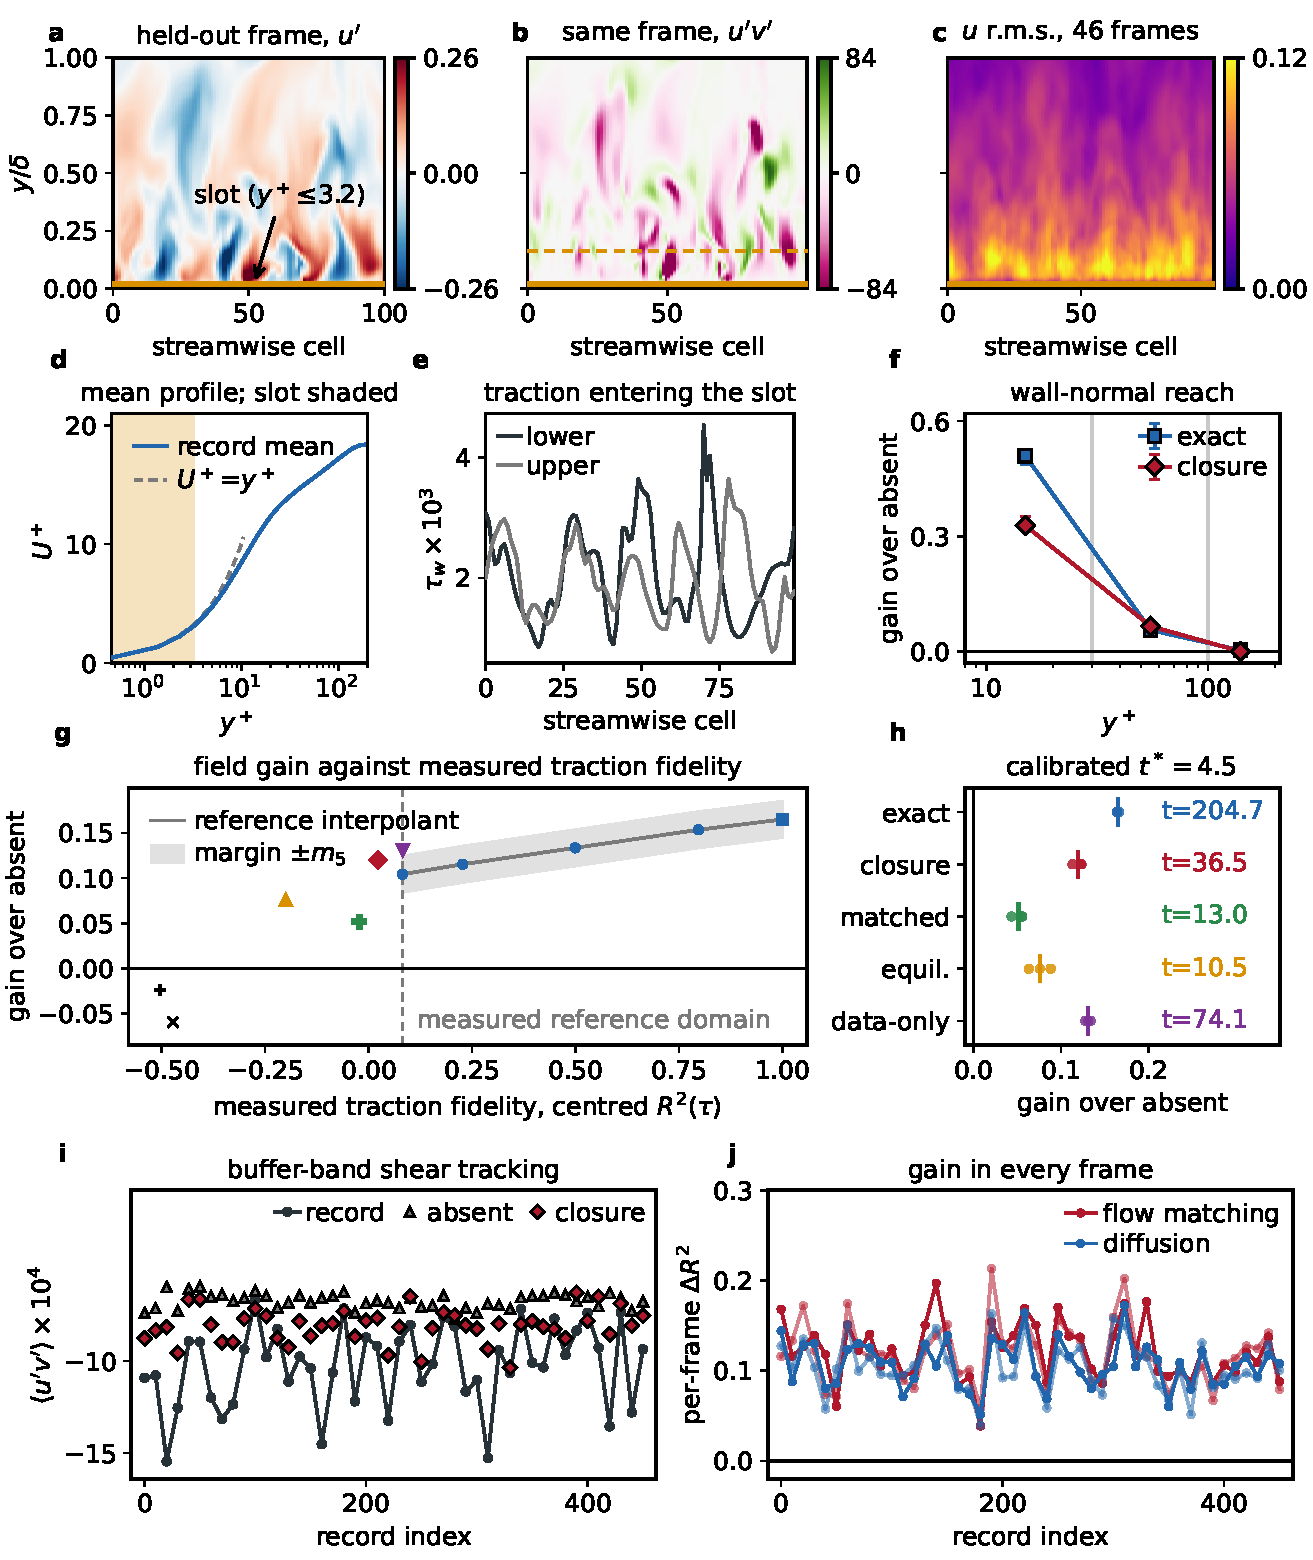
\includegraphics[width=\linewidth]{figures/fig14_slot_interface.pdf}
\caption{\textbf{A single-slot channel experiment: transmitted traction information improves
the generated field.} \textbf{a}--\textbf{c}, The wall-resolved record: a held-out frame's
$u'$, its $u'v'$ (buffer band dashed), and $u$ r.m.s.\ over 46 frames; gold marks the
conditioning slot ($y^+\leq3.2$). \textbf{d},\textbf{e}, Mean profile in wall units; slot
traction on both walls. \textbf{f}, Wall-normal reach. \textbf{g}, Field gain against
measured traction fidelity; the lowest rung ($r=0.55$) still correlates
structurally with the true traction. \textbf{h}, Block inference at the calibrated
$t^\ast=4.5$. \textbf{i}, Reconstructed buffer-band turbulent shear tracking:
per-frame error $3.84\times10^{-4}$ (absent), $2.83\times10^{-4}$ (closure),
$2.40\times10^{-4}$ (exact traction). \textbf{j},
Per-frame gain; every frame, seed and family positive.}
\label{fig:slot}
\end{figure}
\FloatBarrier
